\begin{figure}[htbp]
    \begin{subfigure}[b]{0.5\linewidth}
        \centering
        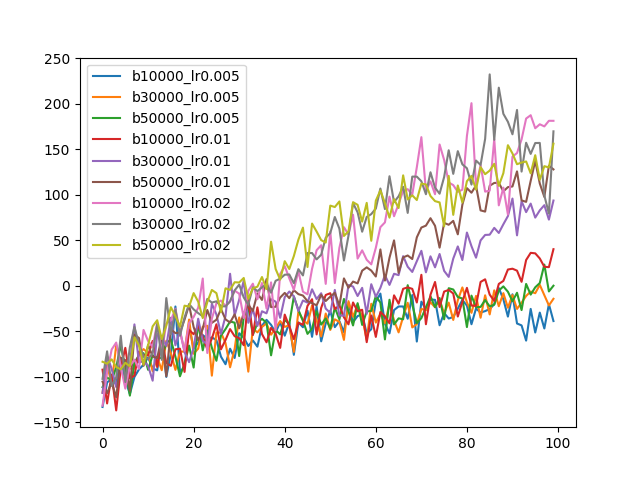
\includegraphics[width=1.0\linewidth]{figures/p7-hyper.png}
        \caption{Hyper-parameter search. }
        \label{fig:p7-hyper}
    \end{subfigure}
    \begin{subfigure}[b]{0.5\linewidth}
        \centering
        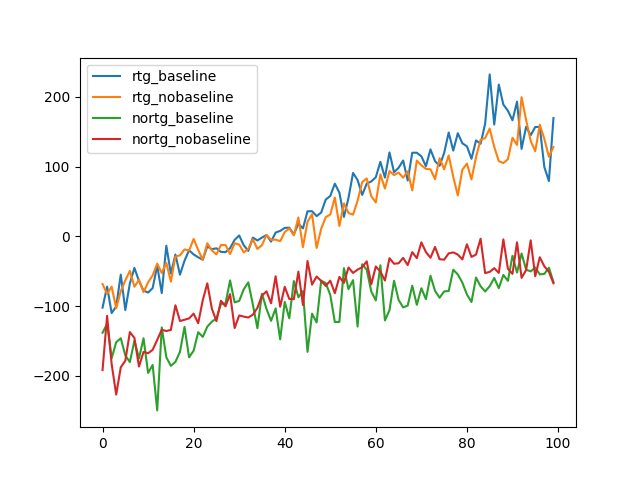
\includegraphics[width=1.0\linewidth]{figures/p7-final.png}
        \caption{With batch size 30k, learning rate $0.02$.}
        \label{fig:p7-final}
    \end{subfigure}
    \caption{Problem 7.}
\end{figure}

See Figure~\ref{fig:p7-hyper} and Figure~\ref{fig:p7-final}. In general, using large learning leads to faster convergence, and using larger batch size also has this effect, but not obvious in some cases. Using neural baseline seems to help, but not much.
